\documentclass[12pt]{article}
\usepackage[english]{babel}
\usepackage[pdftex]{graphicx}
\usepackage[latin1]{inputenc}
\usepackage{verbatim}
\usepackage{listings}
\usepackage{amsfonts}
\usepackage{color}
\usepackage{epsfig}
\usepackage{fancyvrb}
\usepackage{listings}
\usepackage[colorlinks=true, linkcolor = black, urlcolor  = black, citecolor = black, filecolor = black ]{hyperref}
\date{}

\lstset{
  %backgroundcolor=\color{gray},
  frameround=fttt,
  stringstyle=\ttfamily,
  language=python,
  basicstyle=\small
}

\newcommand{\bigtilde}{$\sim$}
\definecolor{unih}{RGB}{1, 178, 170}
%% \def\framework{\textsc{Report}}

%\advance\textwidth by -1truecm
%\advance\oddsidemargin by 1truecm
%\advance\baselineskip by \baselineskip

\begin{document}

\begin{titlepage}
%%   \pagecolor{unih}
  \begin{center}
%%    \textbf{\uppercase{University of HertfordShire}}\\
%%     \hbox to \textwidth{\hrulefill}    
    %\fbox{
    \uppercase{ \textsf{
        \LARGE{REAR} \\ 
        \vspace{0.5truecm}
        \large{an exocentric vision framework for mobile robot teleoperations}
    }}
    %}              
    \hbox to \textwidth{\hrulefill}
    \vfill
    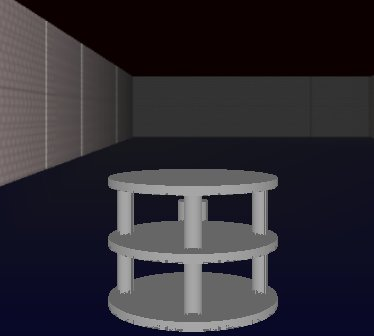
\includegraphics[width=250pt]{img/rear_snapshot.jpg}
    \vfill
    
    \begin{flushright}
      \textsf{Students:} \\
      \textsf{\textbf{Daniele Ferro}} \\                      
      \textsf{\textbf{Loris Fichera}}
      \vspace{0.5 truecm}
                
      \textsf{Supervisor:} \\
      \textsf{\textbf{Prof. Salvatore Livatino }}\\
      \textsf{\textbf{Prof. Giovanni Muscato }}\\
    \end{flushright}
    
    \vspace{0.5 truecm}
    %%    \begin{figure}
    \hfill 
\includegraphics[width=300pt]{img/uni_logo.jpg}  %logo
%%    \end{figure}
    
  \end{center}
  
\end{titlepage}

\setlength{\baselineskip}{1.3\baselineskip} %per 30 righe in ogni pag.

\tableofcontents

\newpage
  % Frontpage
\section{State of the art}
\label{stateart}
%

%
Display used for common Head Mounted Display (HMD) are 
various, we try to explain the chief differences. In the
following we will examine five types: LCD, AMLCD, LCOS, 
FLCOS, OLED.
%

%
\subsection{LCD}
The LCD technology is based on the light modulating properties 
of liquid crystals (LCs). Since LCs are not able to emit light 
directly, actual LCD panels and displays need a light source.
%
That is why such devices are often classified as "passive" 
displays. 
%
LCD displays are usually for a general purpose use, but they 
can also be tuned for a specific usage - e.g. the displaying 
of highly detailed still images or of highly dynamic, 
fast-changing video content.
%
Because of their versatility, they are used in a wide range 
of applications including computer monitors, TVs, aircraft 
cockpits. They're also common in electronic consumer devices 
such as video player, gaming devices, etc.
%
Compared to other display-making technologies - such as CRT - 
LCD allows to make wider and flatter displays while reducing 
electrical power consumption and, thus, making LCD displays 
also well-suitable for mobile devices.
%

%
\subsection{AMLCD}
Active Matrix LCDs (AMLCD) use a matrix of thin-film transistors 
(TFTs) to achieve better performance compared to normal LCD screens. 
They still have polarizing sheets and cells of liquid crystal 
(same as LCD), but the TFTs allow to store the electrical state 
of each pixel on the display while all the other pixels are 
being updated.
%
The advantages of a TFT-LCD monitor are many. It provides a 
larger viewing-angle and a much brighter display than a passive 
matrix monitor with the same size. Some designs have replaced 
transistors with other components such as diodes.
%
With an active matrix only the desired pixel receives a charge, 
acting as a capacitor and holding the charge until the next refresh 
cycle (transistors have the ability to hold a charge for a limited 
period of time). On the contrary, a passive matrix display delivers 
current to the liquid crystals in a specific area with a simple 
conductive grid. AMLCD can be more accurate because, thanks to 
the switching action of transistors, only a the specific pixels 
receive a charge, improving image quality with respect to a 
passive matrix display.
%
AMLCDs are most popular type of display on the market today.

\subsection{LCOS}
Liquid crystal on silicon (LCOS) is a {\it micro-projection} or 
{\it micro-display} technology typically applied in projection 
televisions. It is a reflective technology and uses liquid crystals.
%
LCoS displays are well-suited for high resolution and high contrast 
images. 
%
There are two broad categories of LCoS displays: three-panel and 
single-panel. In three-panel designs, there is one display chip 
per color, and the images are combined optically. Single-panel 
designs, instead, makes use of only one display chip  that shows 
the red, green, and blue components in succession with the 
observer's eyes relied upon to combine the color stream. 
%
If the frequency of the color fields is lower than about 540 Hz, 
an effect called "color breakup" is seen, where false colors 
are briefly perceived when either the image or the observer's 
eye is in motion.
%

%
\subsection{FLCOS}
FLCOS devices are made using ferroelectric liquid crystals 
(so the technology is named FLCoS), which are inherently faster 
than other types of liquid crystals.
%

%
\subsection{OLED}
The Organic Light Emitting Diode (OLED) takes advantage of an 
electroluminescent layer, made of organic compounds, used 
like a LED. This layer is wrapped between two electrodes and 
at least one of the electrodes is transparent.
%
OLEDs are a young display technology, not yet able to emit as 
much light per unit area as an inorganic solid-state based LED. 
For this reason OLED are not used as point-light sources.
%
This devices can be used for multiple applications, from 
television and computer screens to small and portable system 
screens such as mobile phones, PDAs and head-mounted displays 
(where high-resolution is needed).
%
Since OLED displays do not require a backlight, they can 
perform deep black levels and be thinner and lighter than 
LCD panels. Besides, OLED displays can achieve higher contrast 
ratios. Even the power drain is lower, compared to LCD screen.
%

%
\subsection{A comparison towards displays}
By using AMLCD display for Head Mounted Display (HMD) the entire 
device is more compact, because AMLCDs only need a flat backlit 
panel rather than a complex (and thicker) illumination unit. 
This is the reason why FLCOS and LCOS displays are commonly not used. 
%
On the other hand, AMLCD display has relatively low contrast ratio 
and provides the lowest luminance range and largest pixel dimensions 
among all of the previously seen technologies.
As well as AMLCD, OLED offer a compact system design due to its 
self-emission nature. In addition, OLEDs provide a good range of 
luminance, even tough the resolution and contrast ratio of 
existing OLEDs are relatively low compared with FLCOS and LCOS microdisplays.
%
Besides, OLEDs life span would be shortened if the display 
luminance is high (e.g. more than 100 cd/m2).
%
According to \cite{Zhang:08}, for HMD designs a display panel around 2.50 cm is 
preferable as it would offer a good balance of compactness and the 
focal length range of the optics. In fact, when dealing with small 
display panels, shorter focal length and larger magnification are 
required in order to achieve a reasonable field-of-view (FOV). 
%
LCOS microdisplays offer the highest resolution and contrast compared 
with other types of displays and they are commonly used as image 
sources in digital projectors. 
%

%
\begin{figure}[!h]
  \begin{center}
    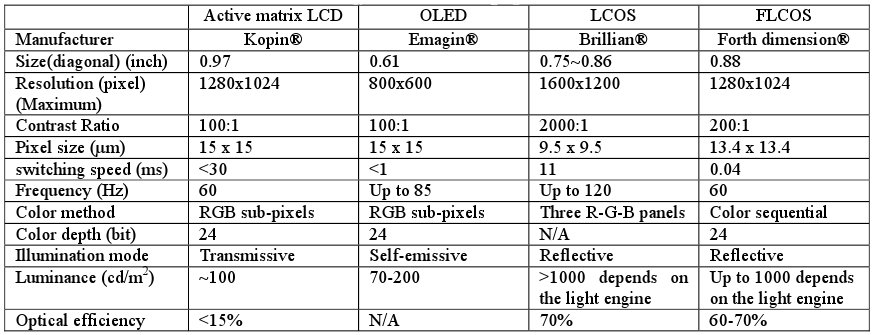
\includegraphics[width=400pt]{img/hmd_comparison_table}  %logo
  \end{center}
\end{figure}
%

%
The liquid crystal used in LCOS microdisplays, however, has low 
switching speed, which makes it impossible to use color sequential 
method, to achieve a full color mode. FLCOS offers high pixel 
resolution, luminance output, image contrast, and optical efficiency. 
Also, the fast response speed of ferroelectric liquid crystal makes 
it possible to achieve full-color display using a single-panel color 
sequential scheme. On the other hand, it requires a carefully designed 
illumination unit to achieve high contrast and high luminance, which 
makes the overall display system less compact than a system using 
AMLCD or OLED microdisplays.

\setcounter{figure}{0}
\setcounter{table}{0}
\setcounter{lstlisting}{0}

\section{The Exocentric vision issue}
\label{sec:exo}

\section{Why exocentric vision ?}
\label{exo:why_exocentric}

Teleoperated mobile robots prove to be extremely useful 
when there is the need for performing operations in places that 
are inaccessible or dangerous for human beings - e.g. 
search-and-rescue missions within unknown regions or into 
collapsed buildings, caves, etc.
\\
The supervisors' research group has been widely involved 
during the last years in such a field: \cite{livatino2010}.
As testing platform, they have been using \morduc{},
a differential-driven mobile robot - see chapter \ref{intro:3morduc} -
equipped with a pair of \textit{Videre Design} \cite{videredesign} 
stereo cameras and a laser scanner.
\\
They have been focused 
mainly on the making of a reliable hardware and software 
infrastructure which could make a remote operator able to drive 
the \morduc{} in comfort.
\\
Indeed, our work focuses on \textit{robot-operator interaction} and, 
hence, on how to improve such interaction. 
\\
Analyzing previous work and data produced by the supervisors' 
research group, it emerges that the stereo cameras mounted on 
top of \morduc{} were used to provide the remote operators a 
\textit{first-person} point of view. In literature, such a 
system is also called an \textit{egocentric} vision system.
\\
According to \cite{sugimoto}, \textit{by observing the camera image 
without an efficient human interface system, the operator 
tends to misinterpret the robot's position and direction}. This is 
due to the fact that \textit{it's difficult for an
operator not accustomed to the vehicle to estimate the
vehicle's position and direction and the distances to a
target strictly based on camera images from the first person 
viewpoint}.
\\
In order to improve the interaction between the robot and the operator 
an exocentric camera would be effective since it would provide a 
view of the robot in the operating environment and, thus, 
a better understanding of where the robot is located into the
environment and its actual direction.
\\
Unfortunately the use of an exocentric camera is not straightforward: 
for example, it could be mounted on a rear-mounted protuberance of the 
robot, but such a protuberance would terribly limit the robot activity and 
its moving abilities.
\\
To avoid such complications, \cite{sugimoto} proposes 
\textit{Time Follower's}, an approach to provide a \textit{virtual exocentric 
view} of a mobile robot.


\subsection{Time Follower's: an overview}
\label{exo:why_exocentric::time_follower}

Time Follower's aims at providing an exocentric view of a mobile 
robot using an egocentric-mounted camera. The approach is simple: it is 
based on the use of previously recorded first-person images to provide 
comprehensible third-person imagery. A 3D representation of the robot 
is overlapped to such images in order to get the work done. A graphical
representation of the system is depicted in figure \ref{fig:exocentric}, 
while figure \ref{fig:virtualexocentric} shows an example of what appears 
to the end user.
\begin{figure}[!h]
  \begin{center}
    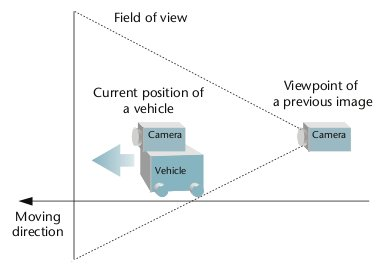
\includegraphics[width=200pt]{img/exocentric_vision.jpg}
    \caption{The \morduc{} robotic platform}
    \label{fig:exocentric}
  \end{center}
\end{figure}

\begin{figure}[!h]
  \begin{center}
    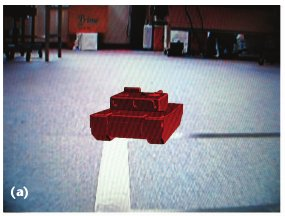
\includegraphics[width=200pt]{img/virtual_exocentric.jpg}  %robot pic
    \caption{A virtual exocentric vision example}
    \label{fig:virtualexocentric}
  \end{center}
\end{figure}

Key issues of such a system are:

\begin{itemize}
\item how to choose the \textit{best} image
\item how to determine the \textit{right} place to draw the robot
\end{itemize}

As for the first issue, the \textit{best} image is the one that allows 
the generation of the \textit{most comprehensible} external robot view.
\cite{sugimoto} provides a set of three effective metrics to 
determine which, of a set of previously recorded images, is the 
one to be chosen.
\\
Once the image is chosen, where to overlap the 3D robot representation 
is quite complex. It is not only a matter of \textit{where} draw the robot
on the image, but also of \textit{how} to set up lighting, robot dimensions,
perspective to make the end user not aware of the fact that what he is
seeing is not the actual environment.
\\
The issues introduced above will be deeply analyzed in the following 
of this document.

\newpage

\section{Time Follower's: an overview}
\label{exo:time_follower}

Time Follower's aims at providing an exocentric view of a mobile 
robot using an egocentric-mounted camera. The approach is simple: it is 
based on the use of previously recorded first-person images to provide 
comprehensible third-person imagery. A 3D representation of the robot 
is overlapped to such images in order to get the work done. A graphical
representation of the system is depicted in figure \ref{fig:exocentric}, 
while figure \ref{fig:virtualexocentric} shows an example of what appears 
to the end user.

\begin{figure}[!h]
  \begin{center}
    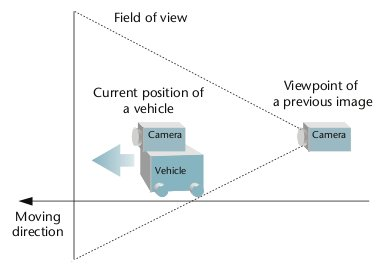
\includegraphics[width=200pt]{img/exocentric_vision.jpg}
    \caption{The Morduc robotic platform}
    \label{fig:exocentric}
  \end{center}
\end{figure}

\begin{figure}[!h]
  \begin{center}
    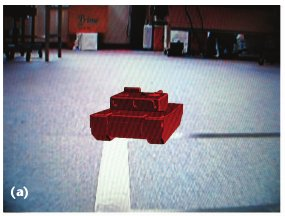
\includegraphics[width=200pt]{img/virtual_exocentric.jpg}  %robot pic
    \caption{A virtual exocentric vision example}
    \label{fig:virtualexocentric}
  \end{center}
\end{figure}

Key issues of such a system are:

\begin{itemize}
\item how to choose the \textit{best} image
\item how to determine the \textit{right} place to draw the robot
\end{itemize}

As for the first issue, the \textit{best} image is the one that allows 
the generation of the \textit{most comprehensible} external robot view.
\cite{sugimoto} provides a set of three effective metrics to 
determine which, of a set of previously recorded images, is the 
one to be chosen.
\\
Once the image is chosen, where to overlap the 3D robot representation 
is quite complex. It is not only a matter of \textit{where} draw the robot
on the image, but also of \textit{how} to set up lighting, robot dimensions,
perspective to make the end user not aware of the fact that what he is
seeing is not the actual environment.
\\
The issues introduced above will be deeply analyzed in the following 
of this document.



\section{Setting up a 3morduc simulator}
\label{sec:simulator}

In order to implement the exocentric vision \ref{sec:exo} we need a wide set of data provided by the robot.
This information consists of the camera images (the egocentric point of view) and of a simple textual file filled with 
the robot status. The latter let us know the robot position and its odometric data, because it would be impossible to draw 
the robot with Augmented Reality (AR) without this knowledge.
\newline The exocentric vision operates better with a large static space where the robot can move in. Since the real robot 
(named 3morduc) can not be easily teleguided in wide environment because of its size and the lack of a large room in Catania, 
where the robot is situated, a simulator has been used to reproduce the best set of data. The simulator can be thought of as 
a server, which receives requests and returns responses: the first are the commands sent by the user to move the robot, the
latter the egocentric images and the robot position data.
\newline Furthermore, with a simulator is extremely easy to change the environment where the robot is teleguided, so we can test
the exocentric vision with an infinite number of environments without physically moving the robot in different places. In this way
software development of exocentric vision can be faster, because it is simple and immediate to establish several test cases.
\newline The first simulator adopted was named 'Rosen'. Written in Erlang language, Rosen has been developed at the University
of Catania in order to simulate the behavior of robot with features completely different from 3morduc. The chief one was that
the robot had its own algorithm to set its movement, it was indeed not guided by a human operator.
\newline Rosen was used a couple of years ago for robot taking part in Euro-robot competition, but for our purpose was not fit
since it does not even provide a egocentric vision. The difficulties faced to edit Rosen made us to look for a more suitable
simulator.
\newline In 2006, at the Aalborg University, the Italian student Filippo Privitera wrote a simulator to teleguide the
3morduc robot \cite{privitera}. The simulator reproduces the robot (drawing its physical features) situated in a room with a
variable numbers of walls. Walls' position is specified by the user, by giving the simulator a black and white bitmap image
with the room plane to build the whole environment from.
\newline Besides, Privitera's simulator allows to enable the stereoscopic vision, with anaglyph or polarized method (both 
types are applied on the egocentric camera). These features make not too tricky to implement the exocentric vision control with 3d
effect, in order to improve the user's ability in moving the robot. Other information like the number of collisions or the robot
distance from the nearest obstacle are provided by simulator.
\newline This simulator was written in MFC (Microsoft Foundation Class) framework and has been used for testing user ability in
driving the robot, in comparison with the real robot server to quantify the differences between the two facilities. For more
information see \cite{privitera}.
\newline With a simulator specifically built for the 3morduc robot, it was not difficult to edit the source code to obtain what we 
needed. First of all, we needed to record data about egocentric vision and robot status, because they are the input value 
of the exocentric vision simulator. In order to achieve this, we edited the source code to allows the user to store data: by
pressing the 'P' key keyboard the actual information (e.g. the actual camera image and robot status) are recorded in
log files.
\newline Every session in Privitera's simulator has its own identifier (a integer number). When the 'P' key is pressed the
simulator write a new line in the text file named 'data< number of session >', creating the file if it does not exist. Each
line contains four float number values, with the following meaning:
\newline
\newline 1. x coordinate
\newline 2. y coordinate
\newline 3. theta value (in radiant s)
\newline 4. timestamp
\newline 
\newline The timestamp refers to the beginning of the simulation.
\newline Beside the text file there are several bitmap files, each for every line written in 'data <number of session>'. These 
files are named 'screenshot<number of session> <timestamp>', where the number of session indicates for every screenshot (e.g.
the egocentric vision) the proper text file, and the timestamp the line with the associated status of the robot.
\newline The software which implement the exocentric vision control will look for text and image files related to a specific 
session, in order to read the necessary input and draw the robot correctly. It must be able to choose the right image to use as 
background, among those previously read; to draw the robot over the background in the right position and orientation, depending 
on its route; to prevent or signal collisions to the user, and so on.
\newline Future development can reach a more interactive collaboration between simulator and exocentric vision control program. For
example, it would be better if the control program could interact (by a socket or another data stream) with the simulator, sending
the movement command and retrieving information about robot status. In this case log files would be substituted by a local or 
global connection, and the exocentric program would not read information from file (as it actually does) but from the network.
Furthermore, with log files the robot route is statically decided when they are created. With a network connection user
could teleguide the robot in real time, without caring if on the server side is present the simulator or the real robot 3morduc.

\section{Introducing OpenGL}
\label{sec:opengl}
\lstset{language=C++}
\subsection{A short introduction to OpenGL}
OpenGL is designed as a software interface to the graphics 
hardware on your computer. It defines a platform-independent API;
the API is then implemented in software and/or hardware for 
various machine architectures. The advantage is that OpenGL 
programs are easily portable to a variety of computers. 
OpenGL provides basic commands to support rendering. 
In particular, OpenGL doesn't provide functionality to support
windows or user interaction (like keyboard presses or mouse 
actions); these features are provided by a separate library called
GLUT (the OpenGL Utility Toolkit). GLUT also provides some 
higher-level features, such as more complex geometrical objects.
%

%
OpenGL is a state machine, which means that you specify various 
states or modes which remain in effect until changed.
Each command that is executed is carried out within the current 
state. States include things like the current window (where
drawing will appear), colour, viewing and projection matrices, 
drawing modes, positions and characteristics of lights,
materials, and features. These elements will not be introduced 
throughout this document, as they are already explained in
various tutorials \cite{opengl:brieftutorial} o manual books 
\cite{opengl:redbook}.
%

%
Nevertheless, it is important to keep the idea of a 
"state machine" in mind as you work with OpenGL in order to 
understand the effects of a given command. The current state 
is not reset when a function starts or ends - the current state
is in effect until something changes it, regardless of where 
in the program the next thing is. 
%

%
In the following, we are going to analyse some peculiar 
aspects of OpenGL. Anyway, this chapter is not intended 
to be an exhaustive guide to OpenGL programming 
- like \cite{opengl:distilled}, \cite{opengl:redbook}, but,
instead, as a collection of short how-to regarding the 
aspects of OpenGL which we have dealt with the most 
during our work. 
%
\subsection{Some notes on OpenGL API functions}
One of the design target of OpenGL was to made its API portable 
among multiple architectures. In order to do so, OpenGL 
designers decided not to make use of polymorphism and inheritance 
when they had to provide multiple versions of the same command 
taking different parameters. They used, instead, the following scheme:
%
\begin{verbatim}
    glCommandName{NTd}()
\end{verbatim}
%
that is, every OpenGL function is preceded by \texttt{gl} and can be 
followed by
%
\begin{itemize}
  \item \texttt{N} \\
    the number of parameters the function takes
  \item \texttt{T} \\
    the parameters type
  \item \texttt{d} \\
    if present, it states that the function takes pointers as arguments
\end{itemize}
%
For example, the \texttt{glVertex} can be invoked as:
\begin{itemize}
\item \texttt{glVertex2i(1, 3)}
\item \texttt{glVertex2f(1.0, 3.5)}
\end{itemize}
%% As you might have observed from the simple program in the preceding
%% section, OpenGL commands use the prefix gl and initial capital letters
%% for each word making up the command name (recall glClearColor(), for
%% example). Similarly, OpenGL defined constants begin with GL_, use all
%% capital letters, and use underscores to separate words (for example,
%% GL_COLOR_BUFFER_BIT).
%% You might also have noticed some seemingly extraneous letters appended to
%% some command names (for example, the 3f in glColor3f() and glVertex3f()).

%% spiegare che non si fa uso di polimorfismo, ma le funzioni
%% hanno un nome specifico a seconda dei parametri che prendono

%
\subsection{The Depth Buffer}
When drawing up a scene with OpenGL, the order in which polygons are drawn
greatly affects the blended result, especially when it comes to 3D.
%

%
The depth buffer keeps track of the distance between the viewpoint and 
the portion of the object occupying a given pixel in a window on the 
screen; when another candidate colour arrives for that pixel, it's drawn 
only if its object is closer to the viewpoint, in which case its depth
value is stored in the depth buffer. With this method, obscured (or hidden)
portions of surfaces aren't drawn and, therefore, aren't used for
blending.
%

%
In order to enable the use of the depth buffer, the 
\texttt{glutInitDisplayMode()} can be used, passing the 
GLUT\_DEPTH macro as an argument.
%

\subsection{OpenGL viewing model}
OpenGL not only provides function to specify models for 
three-dimensional objects but also allows to specify the 
position for each of the models we want to display in a 
scene and also the point from which to view the scene.
%

%
The transformation process used to produce a scene for viewing 
is analogous to taking a photograph with a camera (in fact, it 
is often addressed as \textit{the camera analogy}\cite{opengl:cameraanalogy}) 
and consists of four steps, known as 
\textit{the OpenGL pipeline} (see figure \ref{fig:openglpipe}).
%
\begin{figure}[!h]
  \begin{center}
    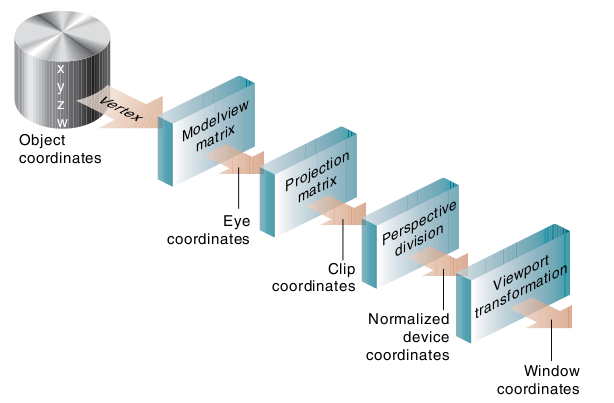
\includegraphics[width=300pt]{img/openGLpipe.png}
    \caption{The OpenGL pipeline}
    \label{fig:openglpipe}
  \end{center}
\end{figure}
%
At the beginning of the pipeline, we have the \textit{raw} 
coordinates of the models we want to put on the scene. Such 
coordinates are then multiplied by the a 4x4 \textbf{modelview} 
matrix, that is, a matrix that stores both \textit{model} and 
\textit{viewing} transformations and which elements have been set 
accordingly to \textit{actually} where to place items in the scene.
%

%
The second step involves the \textbf{projection} matrix, 
which is applied to the incoming object coordinates to define a 
viewing volume. Of course, objects outside this volume are clipped 
so that they are not drawn in the final scene. 
%

%
In the last two steps of the pipe, incoming coordinates are transformed 
into actual two-dimensional window coordinates and other stuff, such as 
the light intensity for each pixel, are calculated according to depth.
%
\subsubsection{Matrix transformations}
To edit the \textbf{modelview} and \textbf{projection} matrices, OpenGL 
provides quite a lot of functions: some of them are 
\textit{general purpose}, that is, they can be used to edit both of them, 
others are specifically intended to edit either the modelview or the 
projection matrix.
%

%
The most used \textit{general purpose} functions are 
%
\begin{itemize}
\item \texttt{glMatrixMode(GLenum mode)} \\
  \textit{mode} specifies which matrix is the \textit{current}
  matrix, that is, the matrix that is to be edited by following
  functions

\item \texttt{glLoadIdentity()} \\
  sets the \textit{current} matrix to be 4x4 identity matrix
\end{itemize}
%

%
For what concerns editing the \textbf{modelview} matrix, OpenGL 
provides a set of functions that allows the specifying of the 
transformations one would like to apply without manually 
editing the modelview matrix. The most used are 
%
\begin{itemize}
\item \texttt{glTranslate(TYPE x, TYPE y, TYPE z)}\\
  Multiplies the current matrix by a matrix that moves 
  (translates) an object by the given x-, y-, and z-values 
  (or moves the local coordinate system by the same amounts)

\item \texttt{glRotate(TYPE angle, TYPE x, TYPE y, TYPE z)} \\
  Multiplies the current matrix by a matrix that rotates an 
  object (or the   local coordinate system) in a counterclockwise 
  direction about the ray from the origin through the point 
  (x, y, z). The angle parameter specifies the angle of rotation in degrees.
\end{itemize}
Two examples are shown in figures \ref{fig:gltranslate}, \ref{fig:glrotate}:
the first one shows the effects of invoking \texttt{glTranslatef(0.0, 0.0, -5.0)} 
on the view, while the second one shows how to rotate a model of 45 degrees 
invoking \texttt{glRotatef(45.0, 0.0, 0.0, 1.0)}.
%
\begin{figure}[!h]
  \begin{center}
    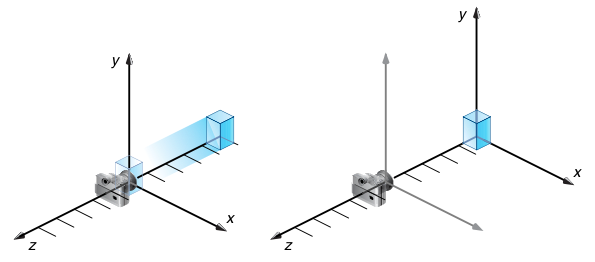
\includegraphics[width=300pt]{img/gltranslate.png}
    \caption{A view transformations by means of a glTranslate invocation}
    \label{fig:gltranslate}
  \end{center}
\end{figure}
%
\begin{figure}[!h]
  \begin{center}
    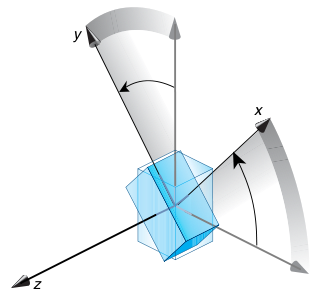
\includegraphics[width=200pt]{img/glrotate.png}
    \caption{A model transformation by means of a glRotate invocation}
    \label{fig:glrotate}
  \end{center}
\end{figure}
%

%
\subsection{Setting up a texture}
According to \cite{opengl:distilled} \textit{texture mapping 
is a concept that takes a moment to grasp but a lifetime 
to master.}
%
As for our work, we were simply interested in drawing an 
image as the background of a window. It is not a complex 
task but, it could be very tricky, especially when one 
does not have a deep understanding of what is happening 
\textit{under the hood}.
%

%
OpenGL provides 1D, 2D and 3D textures. A 2D texture is enough for our
purposes.
%
There exists a well-defined sequence of actions to draw a texture 
into an OpenGL application. Such a sequence made of the following steps:
\begin{enumerate}
\item obtain an unused texture object identifier with \texttt{glGenTextures()}, 
  and create a texture object using \texttt{glBindTexture()}
\item set texture-object state parameters
\item specify the texture image using \texttt{glTexImage2D()} 
  or \texttt{gluBuild2DMipmaps()}
\item before rendering geometry that uses the texture object, 
  bind the texture object with glBindTexture()
\item before rendering geometry, enable texture mapping
\item send geometry to OpenGL with appropriate texture 
  coordinates
\end{enumerate}
%
Let us show an example of how to take a preloaded image, binding it 
to a texture and draw it as the background of a window. First of all, 
we would like to define a helper structure which we will call \texttt{Image}
to store the actual image and its size.
%
\begin{lstlisting}[caption={The Image structure}, label={code:image}, frame=trBL]
struct Image {
  unsigned long sizeX;
  unsigned long sizeY;
  char * data;
};

typedef struct Image Image;
\end{lstlisting}
%
Now, let us suppose to have defined a \texttt{ImageLoad()} function 
that loads an image from disk and returns an object of class \texttt{Image}. 
Let us see how to put in code the procedure described above:
%
\begin{lstlisting}[caption={Texture example}, label={code:texturemapping}, frame=trBL]
  Gluint * texture;
  Image * image;
    
  // allocate space for the image
  image = (Image *) malloc(sizeof(Image));

  if (image == NULL) {
    // ERROR!
    exit(0);
  }

  // load image from disk
  if (!ImageLoad("image.bmp", image)) {
    exit(1);
  }        

  // obtain an unused texture object
  glGenTextures(1, texture);

  // Bind 2d texture (x and y size)
  glBindTexture(GL_TEXTURE_2D, * texture);   

  // now let us set up some state parameters:
  // scale linearly when image bigger than texture
  glTexParameteri(GL_TEXTURE_2D, GL_TEXTURE_MAG_FILTER,
                                 GL_LINEAR);
 
  // scale linearly when image smaller than texture
  glTexParameteri(GL_TEXTURE_2D, GL_TEXTURE_MIN_FILTER,
                                 GL_LINEAR); 

  gluBuild2DMipmaps(GL_TEXTURE_2D, 3, image1->sizeX, 
                    image1->sizeY, GL_RGB, GL_UNSIGNED_BYTE, 
                    image1->data);

  // enable texture mapping
  glEnable(GL_TEXTURE_2D);
  glMatrixMode(GL_PROJECTION);
  glPushMatrix();
  glLoadIdentity();
  glMatrixMode(GL_MODELVIEW);
  glPushMatrix();
  glLoadIdentity();

  // deactivate depth (Z Axis)
  glDepthMask(false);

  glBegin( GL_QUADS );

  // actually map texture
  {
    glTexCoord2f( 0.f, 0.f );
    glVertex2f( -1, -1 );

    glTexCoord2f( 0.f, 1.f );
    glVertex2f( -1, 1.f );

    glTexCoord2f( 1.f, 1.f );
    glVertex2f( 1.f, 1.f );

    glTexCoord2f( 1.f, 0.f );
    glVertex2f( 1.f, -1 );
  }

  glEnd();

  // reactivate depth (Z axis)
  glDepthMask(true);

  glPopMatrix();
  glMatrixMode(GL_PROJECTION);
  glPopMatrix();
  glMatrixMode(GL_MODELVIEW);
  glDisable(GL_TEXTURE_2D);
\end{lstlisting}
%

%
\subsection{Lighting in OpenGL}
As shown in figure \ref{fig:lighting} OpenGL features three types of light:
\begin{itemize}
  \item Ambient light
  \item Diffuse light
  \item Specular light
\end{itemize}
%
\begin{figure}[!h]
  \begin{center}
    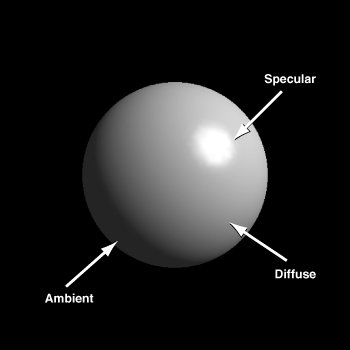
\includegraphics[width=200pt]{img/light}
    \caption{Lighting in OpenGL}
    \label{fig:lighting}
  \end{center}
\end{figure}
%
Ambient light simulates indirect lighting. It illuminates all 
geometry in a scene at the same intensity.
%

%
Diffuse light illuminates a surface based on its orientation 
to a light source. OpenGL diffuse lighting adheres to 
Lambert's law, in which the amount of illumination is proportional 
to the cosine of the angle between the surface normal and the 
light vector, and the diffused light reflects equally in 
all directions.
%

%
Specular light approximates the reflection of the light source on 
a shiny surface.
%

%
At first glance, controlling OpenGL lighting might appear complex. 
The amount of code required to obtain simple lighting effects, 
however, is actually quite small. That is:
\begin{lstlisting}[caption={Lighting example}, label={code:lighting}, frame=trBL]
// Enable OpenGL lighting
glEnable( GL_LIGHTING );

// Enable a single light source
glEnable( GL_LIGHT0 );
\end{lstlisting}
%
\texttt{ GL\_LIGHT0 } is one of the light points available to 
OpenGL programmers. For every light point, one can set its 
position and parameters for each light component. For example:
%
\begin{lstlisting}[caption={Complex lighting example}, label={code:complexlighting}, frame=trBL]
GLfloat lightpos[] = { 0.0f, 0.0f, 1.0f, 0.0f };
GLfloat lightcolor[] = { 1.0f, 1.0f, 1.0f };
GLfloat ambcolor[] = { 1.0f, 1.0f, 1.0f };

glEnable(GL_LIGHTING);
glEnable(GL_LIGHT0);                        
glLightfv(GL_LIGHT0, GL_POSITION, lightpos);
glLightfv(GL_LIGHT0, GL_AMBIENT, lightcolor);
glLightfv(GL_LIGHT0, GL_DIFFUSE, lightcolor);
glLightfv(GL_LIGHT0, GL_SPECULAR, lightcolor);
\end{lstlisting}
%
\subsection{Perspective in OpenGL}
Perspective in OpenGL can be something very trick to work with. 
It all starts from the definition of \textit{frustum}, as the portion
of space seen from the point of view (see \cite{wiki:frustum} 
for further information). To define the frustum we use the function
named \texttt{gluPerspective()} \cite{opengl:gluPerspective}, which takes 
four parameters.
%

%
The first parameter indicates the \textit{FOV} - i.e. Field Of View -
along the Y axis, in degrees: the chosen value is 60. The
second one expresses ratio between actual width and height, 
in our case 624/442. The last two parameters specify the distance 
from the viewer to the near clipping plane and to the far one, 
according to the frustum definition.
%

%
By using two close values for the far and near clipping planes 
distance the application will not be able to display 3d
objects, unless the point of view is relatively close to them. 
If we want to be able to see 3d objects as they are moving away
from the point of view, we need to increase the difference between 
the last two parameters of the \texttt{gluPerspective()} function. In
our case the chosen values are 0.001 and 100000 (its ratio is 
equal to 10exp8).
%

%
The \texttt{gluPerspective()} function affects the \textbf{projection} 
matrix, previously selected by changing matrix mode. Finally,
in order to set our point of view, we must change matrix again, 
this time to work with the \textbf{modelview} matrix.
%

%
The function named
\texttt{gluLookAt()} allows to set the point of view, with its coordinates, 
the coordinates of the point to look at and its orientation.
%

%
See \cite{opengl:gluLookAt} for further details.
%
\begin{lstlisting}[caption={OpenGL perspective example}, label={code:perspective}, frame=trBL]

  /* define the projection transformation */
  glMatrixMode(GL_PROJECTION);
  glLoadIdentity();
  gluPerspective(60, 624/442, 0.001, 100000);
  
  /* define the viewing transformation */
  glMatrixMode(GL_MODELVIEW);
  glLoadIdentity();
  gluLookAt(0.0, 0.0, 10.0,
            0.0, 0.0, 0.0,
            0.0, 1.0, 0.0);

\end{lstlisting}

\subsection{Intro}
\frame
{
  \frametitle{Intro}
  
  \emph{\textit{R.E.A.R.} is a framework for the
    development of \textit{virtual exocentric vision systems}.}
  \pause
  
  \vskip15pt


  \begin{block} {\alert{\texttt{How it works}}}
    \begin{enumerate}

      \footnotesize

      \pause
      \item \texttt{take command input from user}
      \pause
      \item \texttt{send command to robot}
      \pause
      \item \texttt{retrieve robot position \& new egocentric image}
      \pause
      \item \texttt{add image to images' collection}
      \pause
      \item \texttt{choose the proper image to use as background}
      \pause
      \item \texttt{move the camera accordingly to the image chosen}
      \pause
      \item \texttt{move robot in its current position}
      
    \end{enumerate}
      
  \end{block}
      
}

\subsection{Independence from lower details}
\frame
{
  \frametitle{Independence from lower details}
  
  \emph{
    \textit{R.E.A.R.} exploits some object-oriented properties, such as \alert{polymorphism}
    and \alert{inheritance}, in order to work regardless of specific and low level details.
  }

  \vskip10pt
  \pause

  \begin{block} {\alert{\texttt{Lower details}}}
    \begin{itemize}

    \item \alert{\textit{how to draw the robot 3D model}} \\
      \pause

      \vskip5pt
      \only<3>{\footnotesize{user specifies a subclass of \alert{\texttt{Robot}} class: \\

          \begin{description} [\texttt{DrawRobot()}]

            \item [\texttt{DrawRobot()}]
              encapsulates how to draw the robot, through \textit{OpenGL} calls.

          \end{description}
        }}


      \pause

    \item \alert{\textit{how to choose the proper egocentric image}} \\
      \pause

      \vskip5pt
      \only<5>{\footnotesize{user specifies an implementation of \alert{\texttt{IImageSelector}} interface: \\

          \begin{description} [\texttt{ChoseImage()}]

            \item [\texttt{ChoseImage()}]
              encapsulates the exocentric image selection algorithm, given the current
              robot position and previous shot images' set.
          \end{description}
        }}
          
      \pause

    \item \alert{\textit{how to send and retrieve data to/from robot}} \\

      \pause
      \vskip5pt
      \only<7>{\footnotesize{user specifies an implementation of \alert{\texttt{IDataLogic}} interface: \\

          \begin{description} [\texttt{RetrieveData()}]
            \item [\texttt{SelectImage()}]
              delegates exocentric image selection to proper object; 
            \item [\texttt{RetrieveData()}]
              encapsulates how to read new status (i.e. position and egocentric
              image) from robot;
            \item [\texttt{Command()}]
              encapsulates how to send a movement command (forward, backward,
              left, right) to robot.
          \end{description}
        }}

      \pause

    \end{itemize}
    
  \end{block}
}

\setcounter{figure}{0}
\setcounter{table}{0}
\setcounter{lstlisting}{0}

\chapter{Future works}
\label{future_works}
\minitoc

%% This chapter recovers the suggested future implementations scattered in the
%% previous sections, along with some new ideas expressed in a more detailed and
%% uniform way.
%
This section contains some tips for the future development of 
\framework{} and the \textit{sweep metric algorithm}.
%

%
It would be good to make a comparison between the \textit{sweep angle
algorithm} and selection method no. 3 described in \cite{sugimoto}.
%
The formula used in \cite{sugimoto} to compare the view-point of an image with
the robot's current position and direction is not clear at all. Some parameters
are ambiguous and there is not an exhaustive explanation about the formula that
ties them together.
%
After resolving and implementing the formula, it could be interesting to evaluate
the same case tests with the two approaches, in order to underline the advantages
and the disadvantages shown by each method and compare them.
%

%
New implementations of the \texttt{IDataLogic} interface could be 
developed. One could, for instance, interact by a socket or another 
data stream) with the simulator making the whole system working \textit{online}, 
without the need for saved log files and images. Another one could exploit the 
same approach to connect to the actual Morduc. It would also make possible 
to actually operate the robot remotely.
%

%
In both cases, the class implementing \texttt{IDataLogic} must open a communication
channel, in order to send commands to the robot and retrieve its data.
%
If the server contacted is the Morduc itself, the concrete \texttt{IDataLogic} 
implementation must know the Morduc communication protocol (see section 2.4 of 
\cite{morduc:dasero}). Otherwise, if the client communicates with a custom 
simulator, the communication protocol could be chosen by the developer.
%

%
In document \cite{morduc:neri}, Neri and others prove (by several tests) that \textit{3D
vision guarantees a major precision in the teleguide and good performances on the obstacles
avoidance}. An interesting future development could add the stereoscopic vision to a concrete
\framework{} application, in order to merge the advantages brought by the two different
approaches in robot teleguiding.
%

%
To implement 3D vision, the robot server must provide both the right and left camera images,
whereas the OpenGL functions must draw robot in the proper way on the images retrieved, to render
the 3D effect. More details depends on the 3D technologies chosen by the developer: shutter-glasses,
anaglyph, polarized, or other.
%

%
The work presented in this document dis not take into account 
collisions. If the environment the robot moves in presents walls 
or obstacles to avoid, it could be useful to advise user in case 
of an imminent or already happened collision.
%
A signalling system could be implemented once again with OpenGL, therefore 
with augmented reality.The laser value, provided by the Morduc,
could help to understand when and where draw warnings, as shown in 
\cite{morduc:macalusodetommaso}.
%

%
A more simple, but doubtless useful, future upgrade would consists in 
creating a graphical interface, which allows user to define the
\textit{sweep metric algorithm} initial parameters in a more friendly way. 
%
Currently, all these parameters (e.g. the number of log session or the 
optimal distance) are given by command line.
%

%
Last, but surely not least, two suggestions for the 
\textit{sweep metric algorithm} reported in section 
\ref{performance_evaluation:finalconsiderations}.
%

%
An upgraded version of the algorithm could feature a 
\textit{variable} optimal distance value. That value 
could, for instance, be increased when the robot is moving 
along straight lines and could be decreased when it starts 
turning.
%

%
To avoid sudden point-of-view changings during hard turnings, 
a possible solution would be to modify the image selection algorithm 
to have it behaving as follows: when it detects hard turnings, the 
image to be set as background should provide a greater field-of-view. 
In other words, instead of selecting the image provided by the 
egocentric camera, the algorithm should select an image taken 
in a position more distant than the optimal distance.
%


% Bibliography with BibTeX

% see http://www.tex.ac.uk/cgi-bin/texfaq2html?label=tocbibind
% for more details about the following command needed
% for hyperlinking correctly the bibliography
\cleardoublepage
\phantomsection

\addcontentsline{toc}{section}{Bibliography}
\bibliography{biblio}
\bibliographystyle{style/IEEEtran}

\end{document}
